% ==============================================================================
% PHẦN TRÊN: BỐ CỤC 2 CỘT (CỘT LỀ TRÁI VÀ CỘT NỘI DUNG CHÍNH)
% ==============================================================================
\noindent
\begin{minipage}[t]{0.24\textwidth}
    % Cột lề trái để trống theo đúng bố cục bản gốc tại phần này
    \vspace{0pt}
\end{minipage}%
\hfill
\begin{minipage}[t]{0.73\textwidth}
    \vspace{0pt}
    
    % VÍ DỤ 2
    \noindent\textbf{\textsf{\color{stewartcyan}VÍ DỤ 2}}\hspace{1.2em}Mỗi hàm số sau đây gián đoạn tại đâu?
    \vspace{3pt}

    \begin{tabular}{@{}p{0.45\linewidth}@{\hspace{0.05\linewidth}}p{0.50\linewidth}@{}}
    (a)\enspace $f(x) = \dfrac{x^2 - x - 2}{x - 2}$ &
    (b)\enspace $f(x) = \begin{cases}
        \dfrac{x^2 - x - 2}{x - 2} & \text{nếu } x \neq 2 \\[8pt]
        1 & \text{nếu } x = 2
    \end{cases}$ \\[20pt]
    (c)\enspace $f(x) = \begin{cases}
        \dfrac{1}{x^2} & \text{nếu } x \neq 0 \\[8pt]
        1 & \text{nếu } x = 0
    \end{cases}$ &
    (d)\enspace $f(x) = \llbracket x \rrbracket$
    \end{tabular}

    \vspace{6pt}

    % LỜI GIẢI
    \noindent\textbf{\textsf{\color{stewartcyan}LỜI GIẢI}}\hspace{1.2em}\textbf{(a)}\enspace Để ý rằng $f(2)$ không xác định, do đó $f$ gián đoạn tại 2. Sau này chúng ta sẽ thấy tại sao $f$ liên tục tại tất cả các số khác.

    \textbf{(b)}\enspace Ở đây $f(2) = 1$ được xác định và
    \[
    \lim_{x \to 2} f(x) = \lim_{x \to 2} \frac{x^2 - x - 2}{x - 2} = \lim_{x \to 2} \frac{(x - 2)(x + 1)}{x - 2} = \lim_{x \to 2} (x + 1) = 3
    \]
    tồn tại. Nhưng
    \[
    \lim_{x \to 2} f(x) \neq f(2)
    \]
    do đó $f$ không liên tục tại 2.

    \textbf{(c)}\enspace Ở đây $f(0) = 1$ được xác định nhưng
    \[
    \lim_{x \to 0} f(x) = \lim_{x \to 0} \frac{1}{x^2}
    \]
    không tồn tại. (Xem Ví dụ 2.2.6.) Do đó $f$ gián đoạn tại 0.

    \textbf{(d)}\enspace Hàm phần nguyên lớn nhất $f(x) = \llbracket x \rrbracket$ có các điểm gián đoạn tại tất cả các số nguyên vì $\lim_{x \to n} \llbracket x \rrbracket$ không tồn tại nếu $n$ là một số nguyên. (Xem Ví dụ 2.3.10 và Bài tập 2.3.55.)\hfill{\color{stewartcyan}$\blacksquare$}

    \vspace{6pt}

    % Đoạn văn giải thích dưới lời giải
    Hình 3 biểu diễn đồ thị của các hàm số trong Ví dụ 2. Trong mỗi trường hợp, đồ thị không thể vẽ được mà không nhấc bút khỏi mặt giấy vì xuất hiện một lỗ thủng, một chỗ đứt đoạn hoặc một bước nhảy trên đồ thị. Loại gián đoạn được minh họa ở phần (a) và (b) được gọi là \textbf{khử được} vì chúng ta có thể khử điểm gián đoạn bằng cách định nghĩa lại $f$ chỉ tại duy nhất số 2. [Nếu chúng ta định nghĩa lại $f$ bằng 3 tại $x = 2$, thì khi đó $f$ tương đương với hàm số $g(x) = x + 1$, là một hàm liên tục.] Điểm gián đoạn ở phần (c) được gọi là \textbf{gián đoạn vô cực}. Các điểm gián đoạn ở phần (d) được gọi là các \textbf{gián đoạn nhảy} vì hàm số “nhảy” từ giá trị này sang giá trị khác.
\end{minipage}

\vspace{0.8cm}

% ==============================================================================
% PHẦN DƯỚI: HÌNH 3 (TRẢI RỘNG TOÀN BỘ CHIỀU RỘNG TRANG, XÓA NHÃN EN, GẮN NHÃN VN)
% ==============================================================================
\noindent
\begin{minipage}{\textwidth}
    \centering
    \begin{tikzpicture}
        \node[anchor=south west, inner sep=0] (fig) at (0,0) {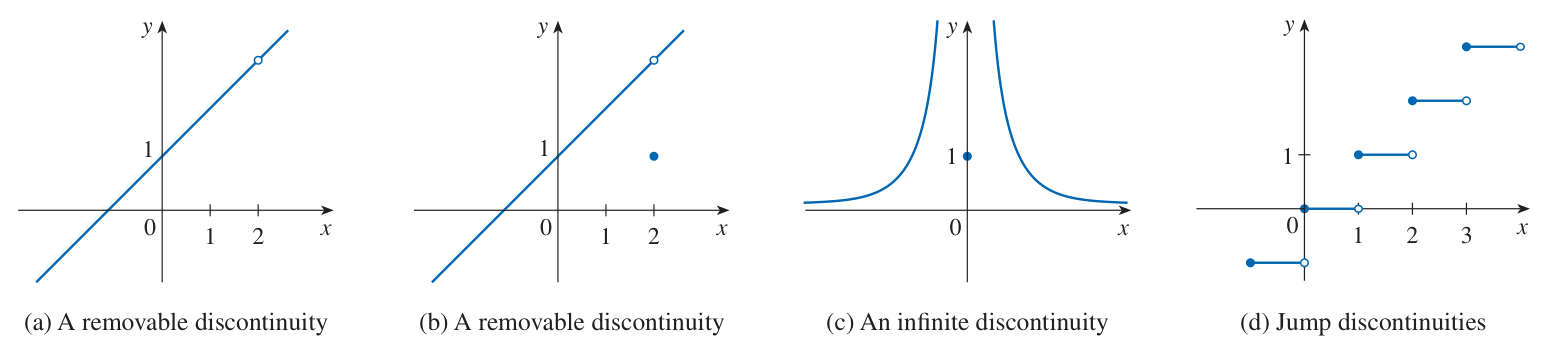
\includegraphics[width=\textwidth]{images/p0151_fig1.png}};
        \begin{scope}[x={(fig.south east)}, y={(fig.north west)}]
            % Phủ trắng che đi phần nhãn tiếng Anh ở đáy ảnh
            \fill[white] (0, 0) rectangle (1, 0.15);
            % Điền nhãn tiếng Việt chuẩn xác tại đúng tọa độ x của từng đồ thị
            \node[anchor=center] at (0.125, 0.07) {\small (a) Gián đoạn khử được};
            \node[anchor=center] at (0.375, 0.07) {\small (b) Gián đoạn khử được};
            \node[anchor=center] at (0.625, 0.07) {\small (c) Gián đoạn vô cực};
            \node[anchor=center] at (0.875, 0.07) {\small (d) Các gián đoạn nhảy};
        \end{scope}
    \end{tikzpicture}
    
    \vspace{4pt}
    
    \noindent
    \begin{minipage}[t]{0.28\textwidth}
        \raggedright
        \textbf{\textsf{HÌNH 3}}\\[1pt]
        \footnotesize Đồ thị các hàm số trong Ví dụ 2
    \end{minipage}\hfill
    \begin{minipage}[t]{0.70\textwidth}
        \vspace{0pt}
    \end{minipage}
\end{minipage}
